\documentclass{standalone}
\usepackage{tikz}
\usetikzlibrary{positioning,shapes,shadows,arrows}

\begin{document}
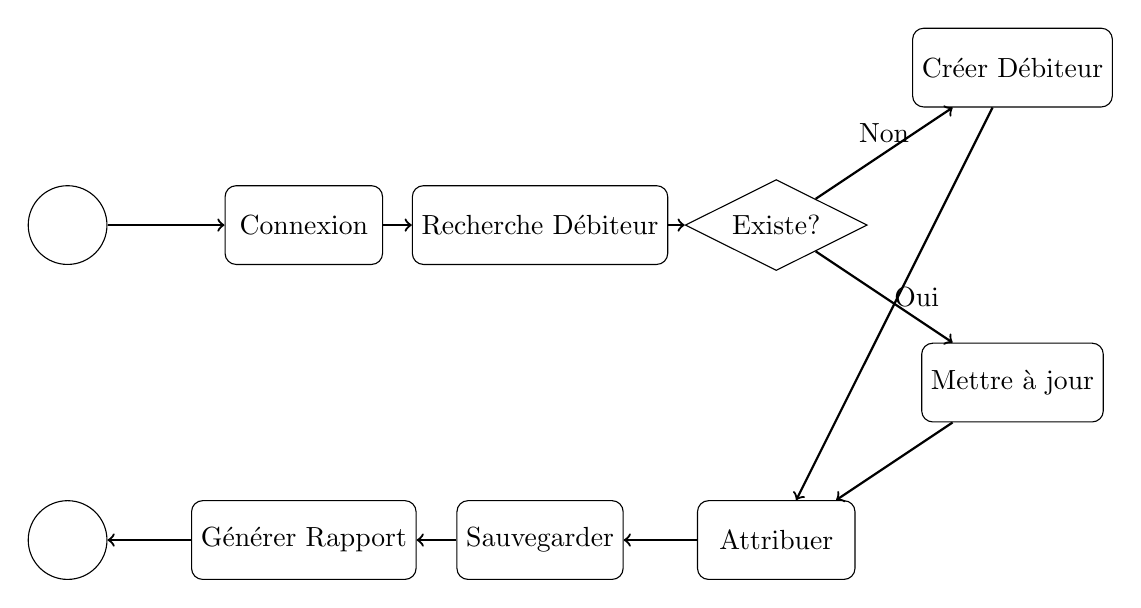
\begin{tikzpicture}[
    activity/.style={draw, rectangle, rounded corners, minimum width=2cm, minimum height=1cm},
    decision/.style={draw, diamond, aspect=2},
    start/.style={draw, circle, minimum size=1cm},
    arrow/.style={->, thick}
]

% Start
\node[start] (start) at (0,0) {};

% Activities
\node[activity] (login) at (3,0) {Connexion};
\node[activity] (search) at (6,0) {Recherche Débiteur};
\node[decision] (exists) at (9,0) {Existe?};
\node[activity] (create) at (12,2) {Créer Débiteur};
\node[activity] (update) at (12,-2) {Mettre à jour};
\node[activity] (assign) at (9,-4) {Attribuer};
\node[activity] (save) at (6,-4) {Sauvegarder};
\node[activity] (report) at (3,-4) {Générer Rapport};

% Arrows
\draw[arrow] (start) -- (login);
\draw[arrow] (login) -- (search);
\draw[arrow] (search) -- (exists);
\draw[arrow] (exists) -- node[above] {Non} (create);
\draw[arrow] (exists) -- node[right] {Oui} (update);
\draw[arrow] (create) -- (assign);
\draw[arrow] (update) -- (assign);
\draw[arrow] (assign) -- (save);
\draw[arrow] (save) -- (report);

% End
\node[start] (end) at (0,-4) {};
\draw[arrow] (report) -- (end);

\end{tikzpicture}
\end{document} 